\documentclass[border=5pt]{standalone}
\usepackage{tikz}
\usepackage{amsmath}
\usetikzlibrary{arrows.meta}

\begin{document}
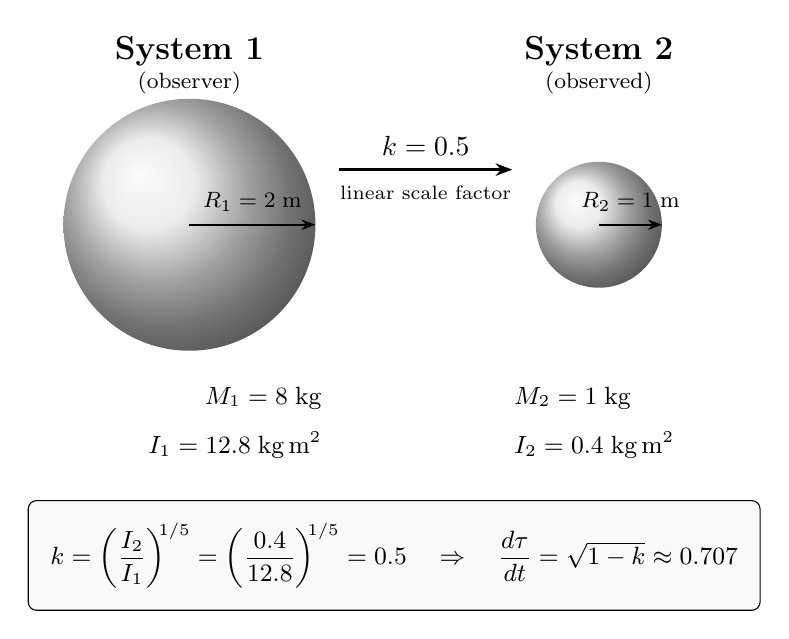
\begin{tikzpicture}

% System 1 (observer) — large sphere, left
\shade[ball color=gray!20] (-2.6,0) circle (1.6cm);
\node[font=\large\bfseries] at (-2.6,2.2) {System 1};
\node[font=\footnotesize] at (-2.6,1.8) {(observer)};
\draw[-{Stealth[length=5pt]}, thick] (-2.6,0) -- (-1.0,0);
\node[font=\footnotesize, above] at (-1.8,0.05) {$R_1 = 2\;\text{m}$};

% System 2 (observed) — small sphere, right
\shade[ball color=gray!20] (2.6,0) circle (0.8cm);
\node[font=\large\bfseries] at (2.6,2.2) {System 2};
\node[font=\footnotesize] at (2.6,1.8) {(observed)};
\draw[-{Stealth[length=5pt]}, thick] (2.6,0) -- (3.4,0);
\node[font=\footnotesize, above] at (3.0,0.05) {$R_2 = 1\;\text{m}$};

% Scale factor between systems
\draw[-{Stealth[length=6pt]}, line width=1.2pt] (-0.7,0.7) -- (1.5,0.7);
\node[font=\normalsize\bfseries, above] at (0.4,0.75) {$k = 0.5$};
\node[font=\scriptsize] at (0.4,0.4) {linear scale factor};

% Properties below System 1
\node[font=\small, anchor=east] at (-0.8,-2.2) {$M_1 = 8\;\text{kg}$};
\node[font=\small, anchor=east] at (-0.8,-2.8) {$I_1 = 12.8\;\text{kg\,m}^2$};

% Properties below System 2
\node[font=\small, anchor=west] at (1.4,-2.2) {$M_2 = 1\;\text{kg}$};
\node[font=\small, anchor=west] at (1.4,-2.8) {$I_2 = 0.4\;\text{kg\,m}^2$};

% STE equation and time dilation result
\node[draw, rounded corners=3pt, fill=gray!5, inner sep=8pt, font=\small]
  at (0,-4.2) {%
    $k = \left(\dfrac{I_2}{I_1}\right)^{\!\!1/5}
       = \left(\dfrac{0.4}{12.8}\right)^{\!\!1/5}
       = 0.5
       \quad\Rightarrow\quad
       \dfrac{d\tau}{dt} = \sqrt{1-k} \approx 0.707$};

\end{tikzpicture}
\end{document}
